\documentclass[12pt,a4paper]{article}
\usepackage[utf8]{inputenc}
\usepackage[top=1.6cm,bottom=1.8cm,left=2.3cm,right=1.8cm]{geometry}
\usepackage{graphicx}
\usepackage{array}
\usepackage{tabularx}
\usepackage{setspace}
\usepackage{mathptmx}
\usepackage{xcolor}
\usepackage{fancyhdr}
\usepackage{enumitem}
\usepackage{multirow}
\usepackage[colorlinks=true,urlcolor=blue,linkcolor=black]{hyperref}

\pagestyle{fancy}
\fancyhf{}
\renewcommand{\headrulewidth}{0pt}
\cfoot{\thepage}

\newcommand{\kopsurat}{%
\noindent
\begin{minipage}[c]{0.14\textwidth}
  \raggedright
  
\includegraphics[height=1.7cm]{telkom_logo.png}
\end{minipage}%
\begin{minipage}[c]{0.72\textwidth}
  \centering
  {\fontsize{11pt}{13pt}\selectfont \textbf{UNIT KEGIATAN MAHASISWA}}\\[1.5pt]
  {\fontsize{10.5pt}{12.5pt}\selectfont \textbf{COMMUNITY SUPPORT CENTER TELKOM UNIVERSITY}}\\[1.5pt]
  {\fontsize{8.5pt}{10.5pt}\selectfont Student Affairs, Jalan Telekomunikasi No.1 Dayeuhkolot,}\\[1pt]
  {\fontsize{8.5pt}{10.5pt}\selectfont Bandung, Jawa Barat 40257}\\[1pt]
  {\fontsize{8.5pt}{10.5pt}\selectfont Email: \textcolor{blue}{\underline{csc.telkomuniversity@gmail.com}}}
\end{minipage}%
\begin{minipage}[c]{0.14\textwidth}
  \raggedleft
  
\includegraphics[height=1.7cm]{csc_logo.png}
\end{minipage}
\vspace{3pt}
\hrule height 0.8pt
\vspace{7pt}
}

\begin{document}

% ==================== PAGE 1: COVER ====================
\thispagestyle{empty}
\begin{center}
  \vspace*{0.5cm}
  {\fontsize{16pt}{20pt}\selectfont \textbf{PROPOSAL KEGIATAN}}\\[0.35cm]
  {\fontsize{18pt}{22pt}\selectfont \textbf{PELATIHAN ADMINISTRASI SPARKS VOL. 1}}\\[2.6cm]
  
  
\includegraphics[width=3.4cm]{telkom_logo.png}\\[0.6cm]
  
\includegraphics[width=4.2cm]{csc_logo.png}\\[3.0cm]

  {\fontsize{14pt}{17pt}\selectfont \textbf{TELKOM UNIVERSITY}}\\[0.15cm]
  {\fontsize{14pt}{17pt}\selectfont \textbf{COMMUNITY SUPPORT CENTER}}\\[0.25cm]
  {\fontsize{9.5pt}{12pt}\selectfont Student Affairs, Jalan Telekomunikasi No.1 Dayeuhkolot, Bandung, Jawa Barat 40257}\\[0.6cm]
  {\fontsize{12pt}{15pt}\selectfont \textbf{TAHUN 2026}}
\end{center}
\clearpage

% ==================== PAGE 2: LEMBAR EVALUASI PROPOSAL ====================
\pagenumbering{Roman}
\setcounter{page}{2}
\kopsurat

\begin{center}
  \textbf{\large LEMBAR EVALUASI PROPOSAL}
\end{center}
\vspace{4pt}

\noindent
\begin{tabular}{|p{5.8cm}|p{10.2cm}|}
\hline
\textbf{UKM/HIMA/BEM/}\newline \textbf{DPM/INDIVIDU/LAB} & Community Support Center Telkom University \\ \hline
\textbf{Kegiatan / Tema} & Pelatihan Administrasi Sparks Vol. 1 \\ \hline
\textbf{Tgl Pelaksanaan} & 12 Mei 2026 \\ \hline
\textbf{Pelaksana} & Community Support Center Telkom University \\ \hline
\textbf{Tempat} & Ruang Kelas TULT \\ \hline
\textbf{Tgl Evaluasi} &  \\ \hline
\end{tabular}

\vspace{8pt}
\noindent\textbf{1. Kepala Urusan Kegiatan Mahasiswa}\\
Pendanaan:
\vspace{2pt}

\noindent
\begin{tabular}{|p{5.1cm}|p{5.1cm}|p{5.8cm}|}
\hline
\textbf{Anggaran} & \textbf{Diajukan} & \textbf{Direkomendasikan} \\
Rp. & Rp. 0,00 & Rp. 0,00 \\ \hline
\end{tabular}

\vspace{3pt}
\noindent
\begin{tabular}{|p{8.5cm}|p{7.9cm}|}
\hline
\textbf{Catatan:} & \textbf{Tanda Tangan / Paraf}\\[1.8cm]
 & Ahmad Adli, S.Kom., M.Kom \\ \hline
\end{tabular}

\vspace{8pt}
\noindent\textbf{2. Kepala Bagian Prestasi dan Kegiatan Mahasiswa}\\
Pendanaan:
\vspace{2pt}

\noindent
\hfill
\begin{tabular}{|p{3.8cm}|p{3.8cm}|}
\hline
\textbf{Disetujui} & Rp. 0,00 \\ \hline
\end{tabular}

\vspace{3pt}
\noindent
\begin{tabular}{|p{8.5cm}|p{7.9cm}|}
\hline
\textbf{Catatan:} & \textbf{Ridwan Sukma AlBusyaeri, M.M., CRP}\\[1.8cm]
 &  \\ \hline
\end{tabular}
\clearpage

% ==================== PAGE 3: FORM KONTROL PENGAJUAN ====================
\kopsurat

\begin{center}
  \textbf{\large FORM KONTROL PENGAJUAN PROPOSAL KEGIATAN}
\end{center}
\vspace{4pt}

\noindent
\begin{tabular}{|p{3.8cm}|p{3.4cm}|p{6cm}|p{2.6cm}|}
\hline
\multicolumn{4}{|c|}{\textbf{\normalsize DIREKTORAT KEMAHASISWAAN}}\\[2pt]
\multicolumn{4}{|c|}{\textbf{\small FORM KONTROL PENGAJUAN PROPOSAL KEGIATAN}}\\ \hline
 & \textbf{Tanggal} & \textbf{Catatan} & \textbf{Paraf} \\ \hline
\textbf{MASUK} & & & \\[0.2cm] \hline
\multirow{2}{*}{\textbf{KELAYAKAN PROPOSAL}} & \textbf{Revisi:} & \multicolumn{2}{l|}{\textbf{Paraf:}} \\
 & [~] Ya\quad [~] Tidak & \multicolumn{2}{l|}{} \\[0.15cm] \hline
 & \textbf{Tanggal} & \textbf{Catatan} & \textbf{Paraf} \\ \hline
\textbf{PRESENTASI} & & & \\[0.2cm] \hline
\multicolumn{4}{|c|}{\textbf{ANGGARAN DIAJUKAN}\hfill\textbf{ANGGARAN DIREKOMENDASIKAN}\hfill\textbf{ANGGARAN DISETUJUI}}\\
\multicolumn{4}{|c|}{Rp. 0,00\hfill Rp. 0,00\hfill Rp. 0,00}\\ \hline
\multirow{2}{*}{\textbf{PENGESAHAN}} & \multicolumn{3}{l|}{Kepala Urusan Kegiatan Mahasiswa \hfill Tanggal: \hspace{1.5cm} Paraf:}\\[0.25cm] \cline{2-4}
 & \multicolumn{3}{l|}{Kepala Bagian Prestasi \& Kegiatan Mhs. \hfill Tanggal: \hspace{1.5cm} Paraf:}\\[0.25cm] \hline
\multirow{4}{*}{\textbf{PENCAIRAN DANA}} & Kwitansi & Tanggal: & Paraf:\\[0.15cm] \cline{2-4}
 & Pengajuan Keuangan & Tanggal: & Paraf:\\[0.15cm] \cline{2-4}
 & Pencairan Keuangan & Tanggal: & Paraf:\\[0.15cm] \cline{2-4}
 & Penyerahan Dana & Tanggal: & Paraf:\\[0.15cm] \hline
\textbf{ARSIP} & Tanggal: & Catatan: & Paraf:\\[0.25cm] \hline
\end{tabular}
\clearpage

% ==================== PAGE 4: REKAP PROPOSAL ====================
\kopsurat

\begin{center}
  \textbf{\large REKAP PROPOSAL}
\end{center}
\vspace{6pt}

\noindent
\begin{tabular}{|c|p{4.5cm}|p{10.5cm}|}
\hline
\textbf{NO} & \textbf{DATA} & \textbf{DESKRIPSI} \\ \hline
1 & Nama Kegiatan & Pelatihan Administrasi Sparks Vol. 1 \\ \hline
2 & Penyelenggara & Community Support Center Telkom University \\ \hline
3 & Afiliasi & UKM IMA \\ \hline
4 & Tempat Kegiatan & Ruang Kelas TULT \\ \hline
5 & Jadwal Kegiatan & 12 Mei 2026 \\ \hline
6 & Total Anggaran Kegiatan & Rp. 0,00 \\ \hline
7 & Pengajuan Dana Internal & Rp. 0,00 \\ \hline
8 & Bentuk Kegiatan & Sharing session \\ \hline
9 & Target Kegiatan & Peningkatan kapasitas Marketing Officer melalui sharing session bersama pengurus organisasi mahasiswa yang berpengalaman dalam pengelolaan strategi pemasaran, branding organisasi, publikasi, serta pengembangan media komunikasi \\ \hline
\end{tabular}
\clearpage

% ==================== PAGE 5: DAFTAR ISI ====================
\kopsurat

\begin{center}
  \textbf{\large DAFTAR ISI}
\end{center}
\vspace{8pt}

\noindent
\begin{tabular}{p{14.2cm}r}
\textbf{LEMBAR EVALUASI PROPOSAL} \dotfill & \textbf{II} \\[3pt]
\textbf{FORM KONTROL PENGAJUAN PROPOSAL KEGIATAN} \dotfill & \textbf{III} \\[3pt]
\textbf{REKAP PROPOSAL} \dotfill & \textbf{IV} \\[3pt]
\textbf{DAFTAR ISI} \dotfill & \textbf{V} \\[3pt]
A. Latar Belakang \dotfill & 1 \\[3pt]
B. Nama Kegiatan \dotfill & 1 \\[3pt]
C. Tema Kegiatan \dotfill & 1 \\[3pt]
D. Tujuan Kegiatan \dotfill & 2 \\[3pt]
E. Sasaran Kegiatan \dotfill & 2 \\[3pt]
F. Waktu dan Tempat \dotfill & 2 \\[3pt]
G. Bentuk Kegiatan \dotfill & 2 \\[3pt]
H. Materi Kegiatan \dotfill & 2 \\[3pt]
I. Narasumber Kegiatan \dotfill & 3 \\[3pt]
J. Susunan Acara \dotfill & 3 \\[3pt]
K. Analisis Risiko \dotfill & 3 \\[3pt]
L. Monitoring dan Evaluasi \dotfill & 4 \\[3pt]
M. Struktur Kepanitiaan \dotfill & 4 \\[3pt]
N. Rencana Anggaran Biaya \dotfill & 5 \\[3pt]
O. Penutup \dotfill & 6 \\[3pt]
\textbf{LEMBAR PENGESAHAN} \dotfill & \textbf{7} \\[3pt]
\textbf{LAMPIRAN} \dotfill & \textbf{8} \\
\end{tabular}
\clearpage

% ==================== PAGE 6 (1): LATAR BELAKANG ====================
\pagenumbering{arabic}
\setcounter{page}{1}
\kopsurat

\noindent\textbf{A. Latar Belakang}
\vspace{4pt}

\setstretch{1.15}
Perkembangan organisasi mahasiswa di lingkungan Telkom University menuntut setiap pengurus untuk memiliki kompetensi kepemimpinan, manajerial, komunikasi, serta pemahaman mengenai tata kelola organisasi yang baik. Sebagai Unit Kegiatan Mahasiswa (UKM) yang masih tergolong baru, Sparks perlu melakukan penguatan kapasitas internal agar setiap bidang mampu menjalankan program kerja secara efektif, profesional, dan berkelanjutan.

Salah satu upaya yang dapat dilakukan adalah melalui kegiatan Pelatihan Administrasi Sparks, yaitu forum penguatan tata naskah dinas, penyusunan dokumen resmi, serta sistem kearsipan dan alur birokrasi bersama organisasi mahasiswa di lingkungan Telkom University yang memiliki pengalaman dan praktik terbaik dalam tata kelola administrasi. Melalui kegiatan ini, pengurus dapat mempelajari sistem kerja kesekretariatan, standarisasi proposal, penyusunan RAB yang akuntabel, teknik penyusunan LPJ, hingga penyelesaian berbagai tantangan administratif dalam kepengurusan.

Kegiatan ini juga menjadi wadah untuk memperluas jejaring antarlembaga kemahasiswaan sehingga tercipta kolaborasi yang saling mendukung dalam pengembangan organisasi. Dengan adanya transfer pengetahuan mengenai administrasi dan kesekretariatan yang tertib, diharapkan setiap bidang di Sparks mampu meningkatkan kualitas kinerja serta memberikan dampak yang lebih optimal bagi anggota maupun lingkungan kampus.

Pelaksanaan kegiatan ini mendukung \textit{Sustainable Development Goals} (SDGs) 4: \textit{Quality Education} melalui peningkatan kapasitas pengurus melalui kegiatan pembelajaran nonformal dan tata kelola keorganisasian. Selain itu, kegiatan ini juga mendukung SDGs 17: \textit{Partnerships for the Goals} dengan mendorong kolaborasi antarorganisasi mahasiswa dalam membangun tata kelola organisasi yang lebih adaptif, inovatif, transparan, dan berkelanjutan.

\vspace{6pt}
\noindent\textbf{B. Nama Kegiatan}\\
Pelatihan Administrasi Sparks Vol. 1

\vspace{6pt}
\noindent\textbf{C. Tema Kegiatan}\\
The Foundation Phase
\clearpage

% ==================== PAGE 7 (2): TUJUAN, SASARAN, WAKTU, BENTUK, MATERI ====================
\kopsurat

\noindent\textbf{D. Tujuan Kegiatan}
\vspace{3pt}
\begin{enumerate}[leftmargin=*,itemsep=1pt]
  \item Meningkatkan kapasitas dan kompetensi pengurus sesuai bidang kepengurusan, khususnya di bidang tata kelola administrasi dan kesekretariatan.
  \item Menambah wawasan mengenai tata kelola organisasi dan standarisasi dokumen dinas berdasarkan pengalaman organisasi mahasiswa lain di Telkom University.
  \item Membangun hubungan dan kolaborasi antarorganisasi mahasiswa di lingkungan Telkom University.
  \item Mendorong terciptanya budaya belajar, berbagi pengalaman, dan pengembangan organisasi secara tertib dan berkelanjutan.
\end{enumerate}

\vspace{4pt}
\noindent\textbf{E. Sasaran Kegiatan}
\vspace{3pt}

\noindent
Sasaran kegiatan ini adalah jajaran pengurus Sparks dengan target minimal 80\% peserta mengikuti seluruh rangkaian kegiatan. Kegiatan difokuskan pada peningkatan kapasitas pengurus dalam pengelolaan administrasi naskah dinas, penyusunan proposal, LPJ, serta alur persuratan resmi organisasi melalui sharing session bersama pengurus yang berpengalaman pada bidang tersebut.

\vspace{4pt}
\noindent\textbf{F. Waktu dan Tempat}
\vspace{3pt}

\noindent
Pelatihan Administrasi Sparks Vol. 1 akan dilaksanakan pada:
\begin{tabbing}
\hspace{3.2cm} \= \hspace{0.4cm} \= \kill
Hari, Tanggal \> : \> Selasa, 12 Mei 2026 \\
Waktu \> : \> 19.00 -- 20.30 WIB \\
Tempat \> : \> Ruang Kelas TULT
\end{tabbing}

\vspace{2pt}
\noindent\textbf{G. Bentuk Kegiatan}
\vspace{3pt}

\noindent
Kegiatan Pelatihan Administrasi dilaksanakan dalam bentuk \textit{sharing session} yang menghadirkan organisasi mahasiswa sebagai narasumber sesuai dengan bidang yang menjadi sasaran kegiatan. Kegiatan dikemas secara interaktif melalui pemaparan materi, diskusi, tanya jawab, serta berbagi pengalaman mengenai pengelolaan administrasi organisasi, sehingga peserta memperoleh wawasan yang dapat diterapkan dalam kepengurusan Sparks.

\vspace{4pt}
\noindent\textbf{H. Materi Kegiatan}
\vspace{3pt}

\noindent
Materi yang disampaikan berfokus pada standarisasi naskah dinas organisasi, penyusunan proposal dan RAB yang akuntabel, penyusunan LPJ kegiatan dan keuangan, pengelolaan kearsipan digital, serta
\clearpage

% ==================== PAGE 8 (3): NARASUMBER, RUNDOWN, ANALISIS RISIKO ====================
\kopsurat

\noindent
berbagi pengalaman dalam membangun tata kelola administrasi organisasi mahasiswa yang tertib dan profesional.

\vspace{5pt}
\noindent\textbf{I. Narasumber Kegiatan}
\vspace{2pt}

\noindent
Kegiatan ini menghadirkan perwakilan pengurus organisasi mahasiswa Telkom University yang berpengalaman sebagai narasumber yang akan berbagi pengalaman dan praktik terbaik dalam tata kelola kesekretariatan, administrasi dinas, serta manajemen kearsipan kelembagaan.

\vspace{5pt}
\noindent\textbf{J. Susunan Acara}
\vspace{3pt}

\noindent
\begin{tabular}{|c|c|p{4.2cm}|p{3.2cm}|p{4.2cm}|}
\hline
\textbf{Waktu} & \textbf{Durasi} & \textbf{Kegiatan} & \textbf{Penanggung Jawab} & \textbf{Keterangan} \\ \hline
19.00 -- 19.10 & 10' & Pembukaan & CSC & Pembukaan kegiatan dan perkenalan narasumber \\ \hline
19.10 -- 20.10 & 60' & Sharing Session Administrasi & Narasumber & Penyampaian materi dan berbagi pengalaman \\ \hline
20.10 -- 20.25 & 15' & Diskusi dan Tanya Jawab & CSC \& Narasumber & Sesi diskusi interaktif bersama peserta \\ \hline
20.25 -- 20.30 & 5' & Penutupan & CSC & Penutupan kegiatan dan dokumentasi \\ \hline
\end{tabular}

\vspace{5pt}
\noindent\textbf{K. Analisis Risiko}
\vspace{2pt}

\noindent
\begin{tabular}{ll}
\textbf{Nama Kegiatan} & : Pelatihan Administrasi Sparks Vol. 1 \\
\textbf{Ketua Kegiatan} & : Muhammad Fatah Mubien \\
\textbf{Dosen Pembina} & : 1. Dr. Maulana Rezi Ramadhana, S.Psi., M.Psi., Psikolog \\
 & \phantom{: }2. Jeng Ayu Ning Tyas, S.Sos., M.I.Kom \\
\textbf{Lokasi} & : Ruang Kelas TULT \\
\textbf{Tanggal Dibuat} & : 10 Juli 2026
\end{tabular}

\vspace{4pt}
\noindent\textbf{Penilaian Risiko}
\vspace{2pt}

\noindent
\begin{tabular}{|p{2.5cm}|p{3.2cm}|c|c|c|p{3.8cm}|c|}
\hline
\textbf{Uraian Kegiatan} & \textbf{Identifikasi Risiko} & \textbf{P} & \textbf{A} & \textbf{TR} & \textbf{Pengendalian Risiko} & \textbf{PJ} \\ \hline
Pelaksanaan sharing session & Narasumber datang terlambat atau berhalangan hadir sehingga jadwal berubah & 2 & 2 & 2 & Melakukan konfirmasi jadwal dan komunikasi dengan narasumber sebelum hari pelaksanaan serta menyiapkan penyesuaian alur. & CSC \\ \hline
\end{tabular}
\clearpage

% ==================== PAGE 9 (4): LANJUTAN RISIKO, MONEV, KEPANITIAAN ====================
\kopsurat

\noindent
\begin{tabular}{|p{2.5cm}|p{3.2cm}|c|c|c|p{3.8cm}|c|}
\hline
\textbf{Uraian Kegiatan} & \textbf{Identifikasi Risiko} & \textbf{P} & \textbf{A} & \textbf{TR} & \textbf{Pengendalian Risiko} & \textbf{PJ} \\ \hline
Pelaksanaan sharing session & Kehadiran peserta tidak memenuhi target sehingga tujuan kegiatan kurang optimal & 2 & 2 & 2 & Mengingatkan peserta melalui grup komunikasi dan melakukan konfirmasi kehadiran sebelum kegiatan berlangsung. & CSC \\ \hline
Pelaksanaan diskusi & Diskusi berlangsung melebihi waktu yang telah ditentukan & 2 & 1 & 2 & Mengatur jalannya diskusi dan mengingatkan alokasi waktu selama kegiatan berlangsung. & CSC \\ \hline
\end{tabular}

\vspace{6pt}
\noindent\textbf{L. Monitoring dan Evaluasi}
\vspace{3pt}

\noindent
\begin{tabular}{|p{4.2cm}|p{11.6cm}|}
\hline
\textbf{Tahapan} & \textbf{Uraian} \\ \hline
Sebelum Kegiatan & Melakukan koordinasi dengan panitia dan narasumber terkait konsep kegiatan, waktu pelaksanaan, serta pembagian tugas agar seluruh persiapan berjalan sesuai rencana \\ \hline
Saat Kegiatan & Melakukan pemantauan terhadap jalannya kegiatan untuk memastikan seluruh rangkaian acara terlaksana sesuai susunan acara, materi tersampaikan dengan baik, serta peserta mengikuti kegiatan secara aktif \\ \hline
Setelah Kegiatan & Melakukan evaluasi internal bersama panitia terhadap pelaksanaan kegiatan, menghimpun masukan dari peserta dan narasumber, serta menyusun rekomendasi sebagai bahan perbaikan berikutnya \\ \hline
\end{tabular}

\vspace{6pt}
\noindent\textbf{M. Struktur Kepanitiaan}
\vspace{3pt}

\noindent
\begin{tabular}{|p{4.2cm}|p{11.6cm}|}
\hline
\multicolumn{2}{|l|}{\textbf{Pembina}} \\ \hline
Pembina 1 & Dr. Maulana Rezi Ramadhana, S.Psi., M.Psi., Psikolog \\ \hline
Pembina 2 & Jeng Ayu Ning Tyas, S.Sos., M.I.Kom \\ \hline
\end{tabular}
\clearpage

% ==================== PAGE 10 (5): PANITIA & RENCANA ANGGARAN BIAYA ====================
\kopsurat

\noindent
\begin{tabular}{|p{4.5cm}|p{2.8cm}|p{1.5cm}|p{6.4cm}|}
\hline
\multicolumn{4}{|l|}{\textbf{Penanggung Jawab Kegiatan}} \\ \hline
Daniandra Prayudisty Ilham & 103012300052 & FIF & S1 Informatika \\ \hline
Karina Damayanti & 104012300411 & FEB & S1 MBTI \\ \hline
Iyang Rohaci Wijaya & 104022330014 & FEB & S1 Akuntansi \\ \hline
Nezatama Akbar Prawira & 106012300158 & FIK & S1 Desain Komunikasi Visual \\ \hline
\multicolumn{4}{|l|}{\textbf{Panitia Kegiatan Divisi Inti}} \\ \hline
\textbf{Ketua Pelaksana} & & & \\
Muhammad Fatah Mubien & 105012330133 & FEB & S1 Administrasi Bisnis \\ \hline
\textbf{Sekretaris Kegiatan} & & & \\
Ghaida Najla Azzahira & 106032400179 & FIK & S1 Desain Interior \\ \hline
\multicolumn{4}{|l|}{\textbf{Divisi Acara}} \\ \hline
Fakhra Dhiya Millati & 104042400181 & FEB & S1 Administrasi Bisnis \\ \hline
Wika wulandari & 104012530090 & FEB & S1 MBTI \\ \hline
Aruni Rantika Pandiangan & 607032500015 & FIT & D3 Sistem Informasi Akuntansi \\ \hline
Ridho Zakwan Hakim & 106012330296 & FIK & S1 Desain Komunikasi Visual \\ \hline
\end{tabular}

\vspace{6pt}
\noindent\textbf{N. Rencana Anggaran Biaya}
\vspace{3pt}

\noindent\textbf{Pemasukan}
\vspace{2pt}

\noindent
\begin{tabular}{|c|p{5.5cm}|c|p{3.5cm}|p{3.5cm}|}
\hline
\textbf{No} & \textbf{Nama} & \textbf{Kuantitas} & \textbf{Harga} & \textbf{Jumlah} \\ \hline
1 & -- & -- & -- & -- \\ \hline
\multicolumn{4}{|l|}{\textbf{TOTAL PEMASUKAN}} & \textbf{Rp0,00} \\ \hline
\end{tabular}

\vspace{5pt}
\noindent\textbf{Pengeluaran}
\vspace{2pt}

\noindent
\begin{tabular}{|c|p{5.5cm}|c|p{3.5cm}|p{3.5cm}|}
\hline
\textbf{No} & \textbf{Nama} & \textbf{Kuantitas} & \textbf{Harga} & \textbf{Jumlah} \\ \hline
1 & -- & -- & -- & -- \\ \hline
\multicolumn{4}{|l|}{\textbf{TOTAL}} & \textbf{Rp0,00} \\ \hline
\multicolumn{4}{|l|}{\textbf{TOTAL PENGELUARAN}} & \textbf{Rp0,00} \\ \hline
\end{tabular}

\vspace{5pt}
\noindent\textbf{Rekapitulasi Anggaran Dana}
\vspace{2pt}

\noindent
\begin{tabular}{|c|p{10.2cm}|p{4.5cm}|}
\hline
\textbf{No} & \textbf{Keterangan} & \textbf{Jumlah} \\ \hline
1 & Total Pemasukan & Rp0,00 \\ \hline
2 & Total Pengeluaran & Rp0,00 \\ \hline
\multicolumn{2}{|l|}{\textbf{Total Pengajuan Dana}} & \textbf{Rp0,00} \\ \hline
\end{tabular}
\clearpage

% ==================== PAGE 11 (6): PENGAJUAN DANA & PENUTUP ====================
\kopsurat

\noindent\textbf{Pengajuan Dana}
\vspace{3pt}

\noindent
\begin{tabular}{|c|p{10.2cm}|p{4.5cm}|}
\hline
\textbf{No} & \textbf{Keterangan} & \textbf{Jumlah} \\ \hline
1 & Pengajuan Dana & Rp0,00 \\ \hline
\multicolumn{2}{|l|}{\textbf{Total Pengajuan Dana}} & \textbf{Rp0,00} \\ \hline
\end{tabular}

\vspace{16pt}
\noindent\textbf{O. Penutup}
\vspace{4pt}

\setstretch{1.18}
Demikian proposal kegiatan Pelatihan Administrasi Sparks Vol. 1 ini disusun sebagai pedoman pelaksanaan kegiatan. Besar harapan kami kegiatan ini dapat menjadi sarana peningkatan kapasitas pengurus Sparks melalui proses pembelajaran dan penguatan tata kelola administrasi organisasi di lingkungan Telkom University.

Melalui kegiatan ini diharapkan setiap pengurus mampu mengembangkan kompetensi sesuai bidangnya, memperkuat koordinasi internal organisasi, serta membangun tata kelola organisasi yang tertib dan akuntabel. Atas perhatian, dukungan, dan kerja sama dari seluruh pihak, kami mengucapkan terima kasih.
\clearpage

% ==================== PAGE 12 (7): LEMBAR PENGESAHAN ====================
\kopsurat

\begin{center}
  \textbf{\large LEMBAR PENGESAHAN}\\[2pt]
  \textbf{Pelatihan Administrasi Sparks Vol. 1}\\[2pt]
  Bandung, 11 Juli 2026
\end{center}
\vspace{4pt}

\noindent
\begin{tabular}{|p{5.1cm}|p{5.1cm}|p{5.1cm}|}
\hline
\centering \textbf{Chief Executive Officer} & \centering \textbf{Executive Secretary} & \centering \textbf{Ketua Pelaksana} \tabularnewline
\centering Community Support Center 2026 & \centering Community Support Center 2026 & \centering Pelatihan Administrasi Sparks Vol. 1 \tabularnewline
\centering 
\includegraphics[width=4.5cm]{sig_dani.png} & \centering 
\includegraphics[width=4.5cm]{sig_karina.png} & \centering 
\includegraphics[width=4.3cm]{sig_fatah.png} \tabularnewline
\centering \textbf{Daniandra Prayudisty Ilham} & \centering \textbf{Karina Damayanti} & \centering \textbf{Muhammad Fatah Mubien} \tabularnewline
\centering NIM. 103012300052 & \centering NIM. 104012300411 & \centering NIM. 105012330133 \tabularnewline
\hline
\end{tabular}

\vspace{6pt}
\noindent
\begin{tabular}{|p{16.0cm}|}
\hline
\centering \textbf{Pembina} \tabularnewline
\centering 
\includegraphics[width=14cm]{sig_pembina.png} \tabularnewline
\centering \textbf{Jeng Ayu Ning Tyas, S.Sos., M.I.Kom} \tabularnewline
\centering NIP. 15880067 \tabularnewline
\hline
\end{tabular}

\vspace{6pt}
\noindent
\begin{tabular}{|p{16.0cm}|}
\hline
\centering \textbf{Menyetujui,} \tabularnewline
\centering \textbf{Direktur Kemahasiswaan, Karir dan Alumni} \tabularnewline
\vspace{1.8cm} \tabularnewline
\centering \textbf{Dr. Maulana Rezi Ramadhana, S.Psi., M.Psi., Psikolog} \tabularnewline
\centering NIP. 20820005 \tabularnewline
\hline
\end{tabular}
\clearpage

% ==================== PAGE 13 (8): LAMPIRAN ====================
\kopsurat

\begin{center}
  \textbf{\large LAMPIRAN}
\end{center}
\vspace{4pt}

\noindent\textbf{Lampiran 1: Permohonan Tanda Tangan Pembina}
\vspace{8pt}

\begin{center}
  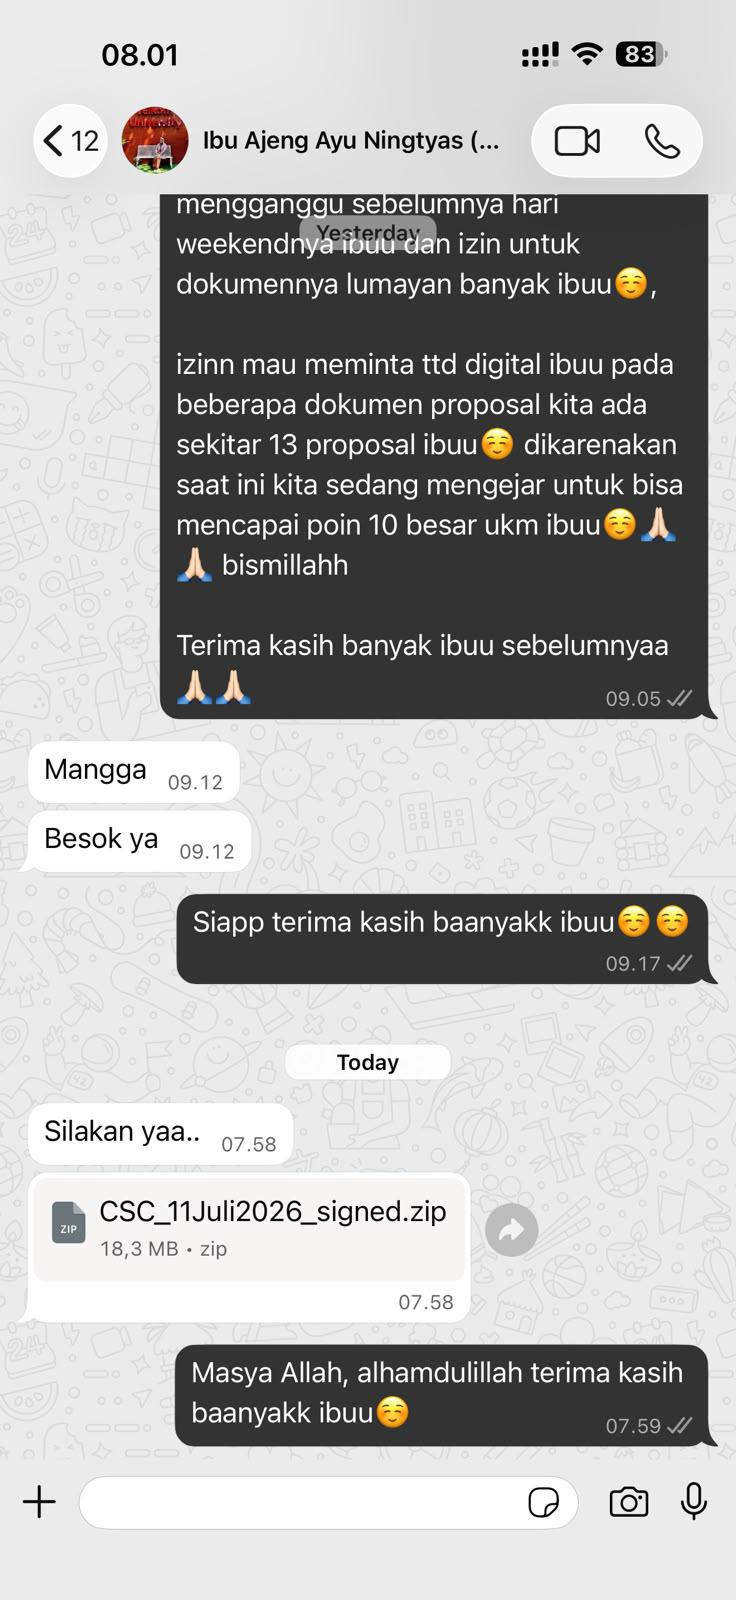
\includegraphics[width=8.5cm]{lampiran_chat.png}
\end{center}

\end{document}
